\label{sec:nueselection:inclusive}

The aim of the inclusive charged-current electron neutrino selection is to select electron neutrinos independently of their final state and energy. The selection performance is approximately 20\%, leading to 250-300 electron neutrino's in the Run 1-4 data-set. The purity without CRT is $\approx 35-40\%$ and with CRT $\approx 45-50\%$.

\subsubsection{Pre-selection}
The selection builds on top of the SliceID (\cref{sec:sliceID}). At first the following cuts are applied:
\begin{itemize}
    \item Reconstructed, space-charge corrected vertex inside a fiducial volume of \SI{10}{\cm} in $x$ and $y$ and $[ \SI{20}{\cm}, \SI{50}{\cm}]$ in $z$.
    \item Topological score above 0.15
    \item CosmicIP $>$ $\SI{15}{\cm}$
    \item slclustfrac $>$ 0.4
    \item An electron candidate shower
\end{itemize}
here, an electron candidate shower is defined as a particle with a trackscore below 0.3, and hits on all three planes. Furthermore, a minimum calorimeric energy of \SI{75}{\MeV} is required. 

At this stage, the efficiency of the selection is 46\% for $\nu_e$ CC events inside the fiducial volume. This is equivalent to 618 events per \SI{10.1e20}{POT}. The number of LEE signal events passing is approximately 30 per \SI{10.1e20}{POT}. The purity at this stage is 3.0\% and the Data/MC ratio is 0.91.

\cref{fig:pre_vtx,fig:pre_shower_E_pdg} show the agreement in the vertex location and kinematics of the electron candidate shower at this stage of the selection. 
%\begin{figure}
%    \centering
%    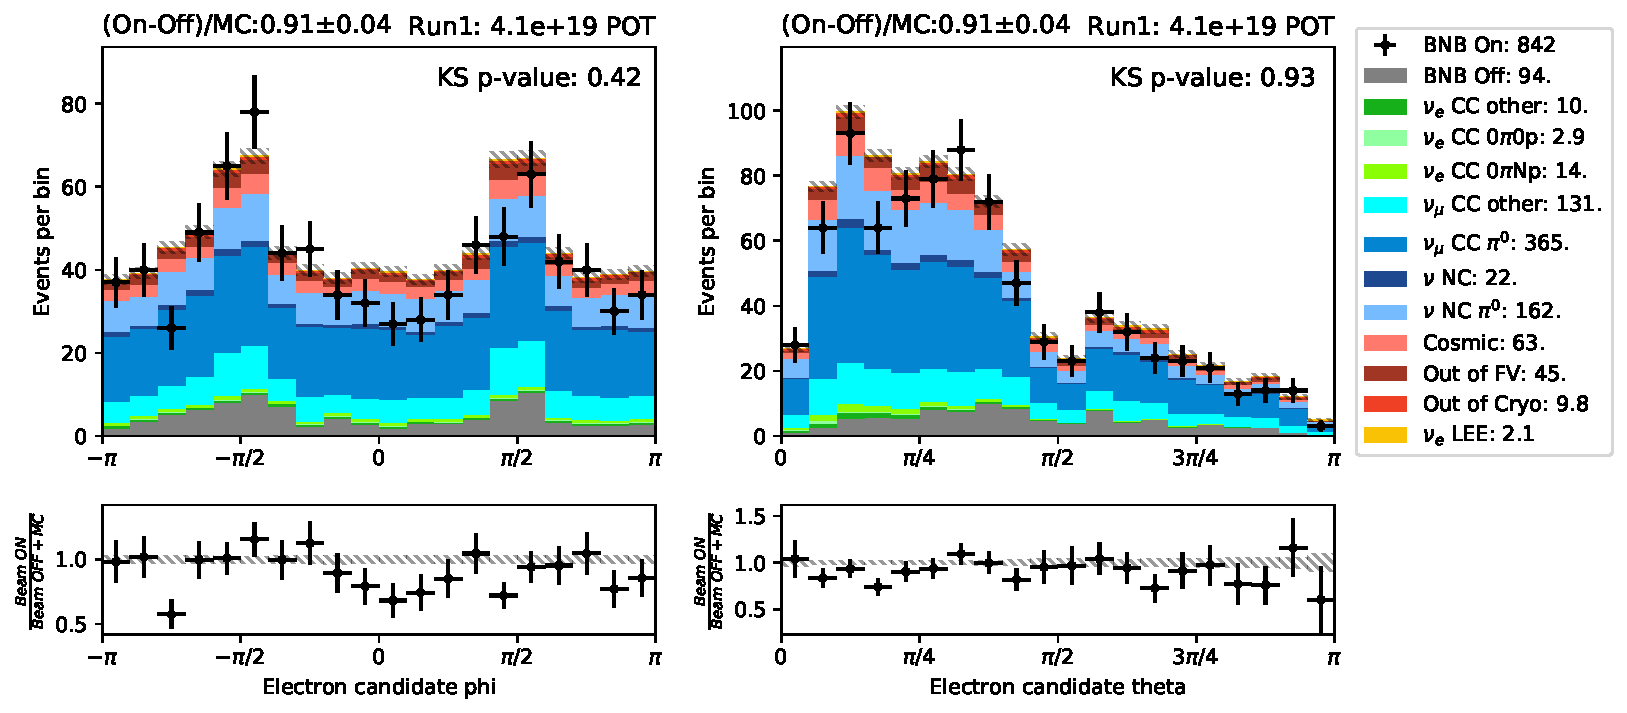
\includegraphics[width=\textwidth]{NueCCsel/Images/run1/pre_angles.pdf}
%    \caption{Caption}
%    \label{fig:pre_shower_E_pdg}
%\end{figure}

\begin{figure}[]
    \centering
    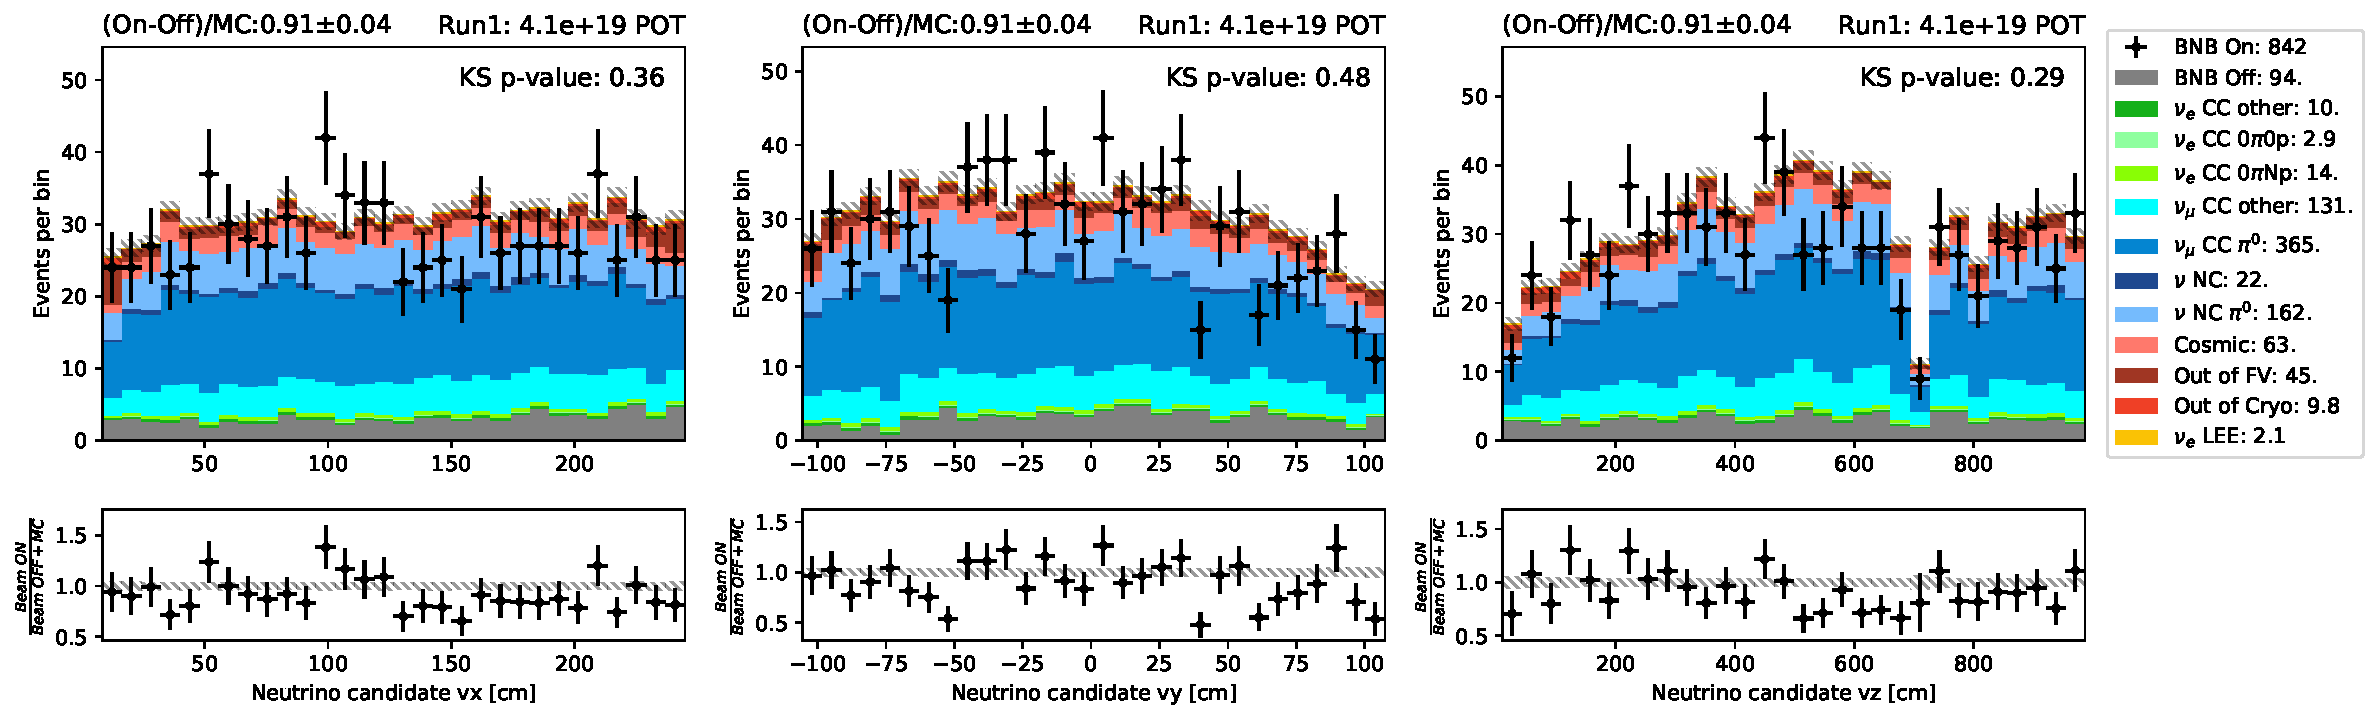
\includegraphics[width=\textwidth]{NueCCsel/Images/run1/pre_vtx.pdf}
    \caption{Vertex position of events passing the pre-selection cuts.}
    \label{fig:pre_vtx}
\end{figure}

\begin{figure}[h]
    \centering
    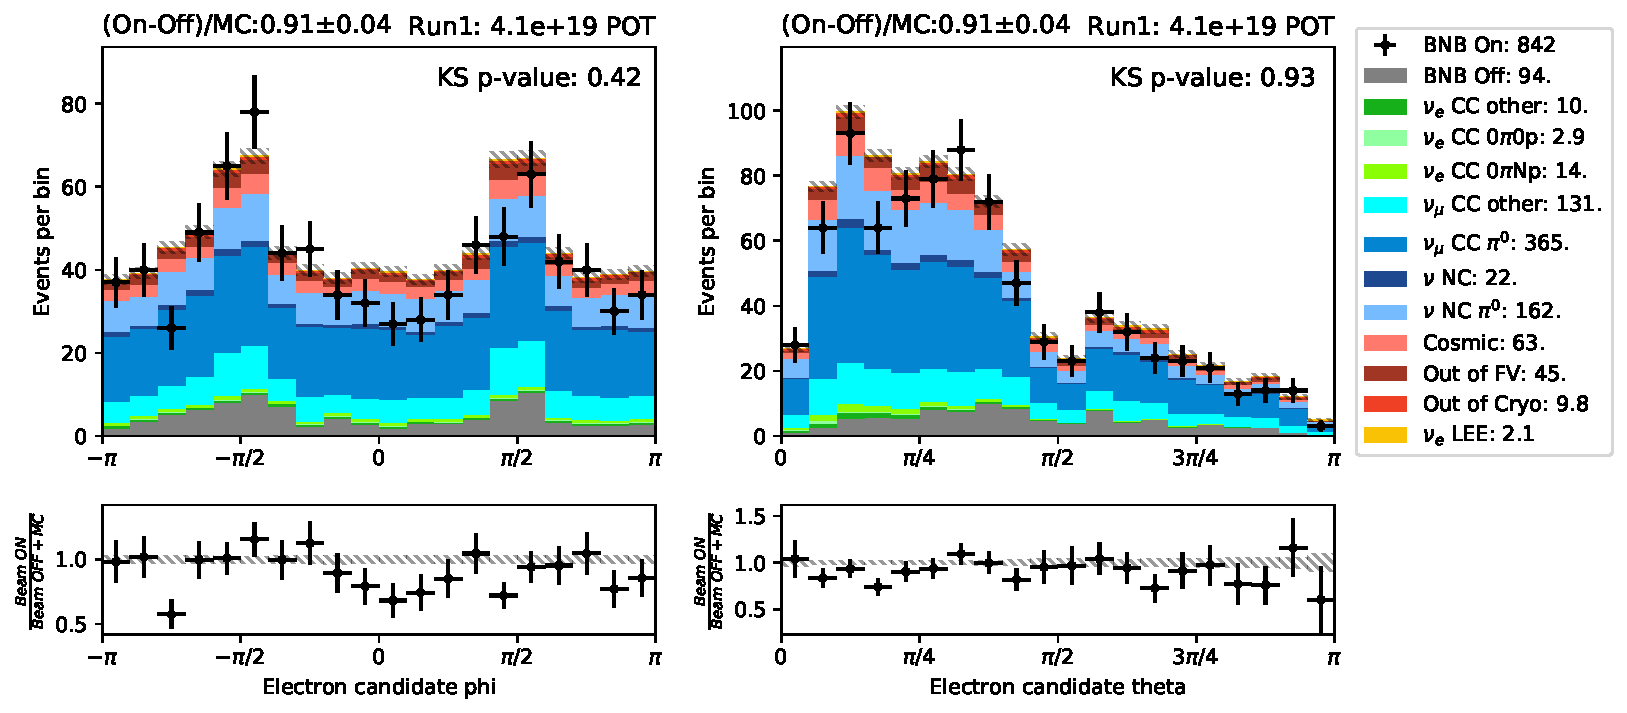
\includegraphics[height=4.9cm]{NueCCsel/Images/run1/pre_angles.pdf}
    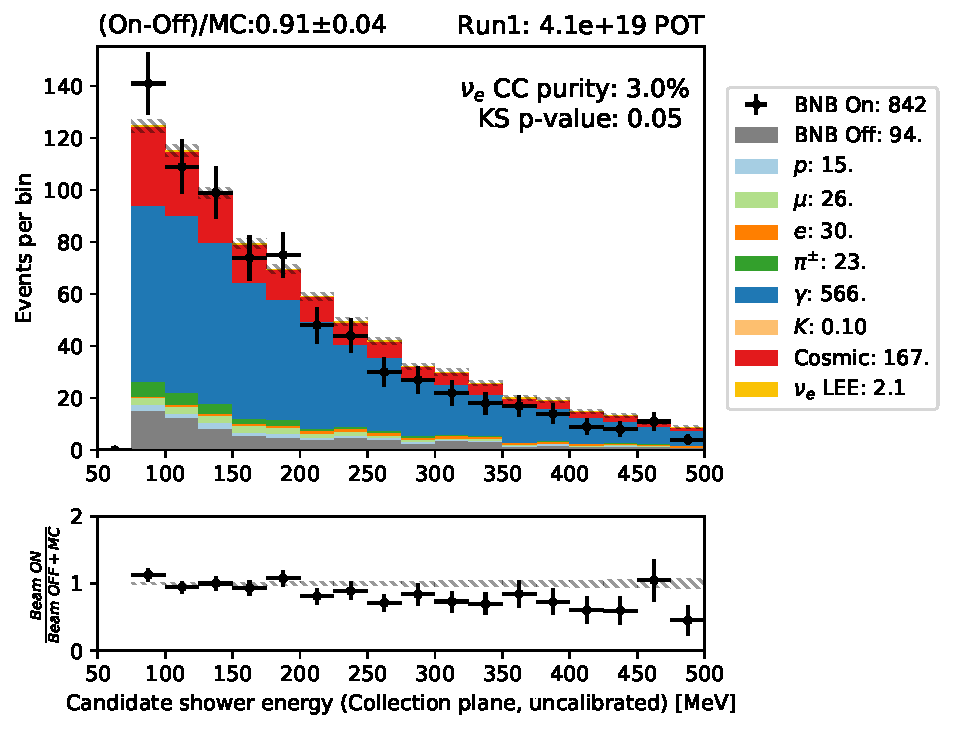
\includegraphics[height=4.9cm]{NueCCsel/Images/run1/pre_shower_E_pdg.pdf}
    \caption{After the pre-selection cuts, the $\nu_e$ CC purity is still low. These panels show the dominant background categories and the distribution of the angles and reconstructed energy of the electron candidate shower. The plot on the right shows that the main background is coming from photons. There is also an indication that the reconstructed energy in MC is slightly overestimated and needs to be corrected.}
    \label{fig:pre_shower_E_pdg}
\end{figure}

\clearpage
\subsubsection{Electron Identification}
After the pre-selection, the object that is tagged as electron candidate is still not an neutrino electron in the dominant fraction of events. The ratio photons to electrons is approximately 20 to 1 and photon-electron separation is therefore the main objective of electron identification. The identification is done using a boosted decision tree, trained on variables that belong to the particle. Those variables are:
\begin{enumerate}
    \item Shower vertex distance.
    \item Shower d$E$/d$x$ at the start of the shower:
    \begin{itemize}
        \item On the collection plane only.
        \item Weighted mean over the 3 planes.
        \item Collection plane, but shifted by \SI{1}{\cm}. 
    \end{itemize}
    \item Shower Moliere radius.
    \item Second shower distance and number of hits on the collection plane.
    \item Number of subclusters in the shower.
    \item ismerged: checks if a proton is merged in the start of the shower.
\end{enumerate}

The three distributions of the variables used to characterise the d$E$/d$x$ at the start of the shower are given in \cref{fig:e_cand_dedx}. The response of the BDT is shown in the right panel of \cref{fig:e_cand_dist}.

\begin{figure}
    \centering
    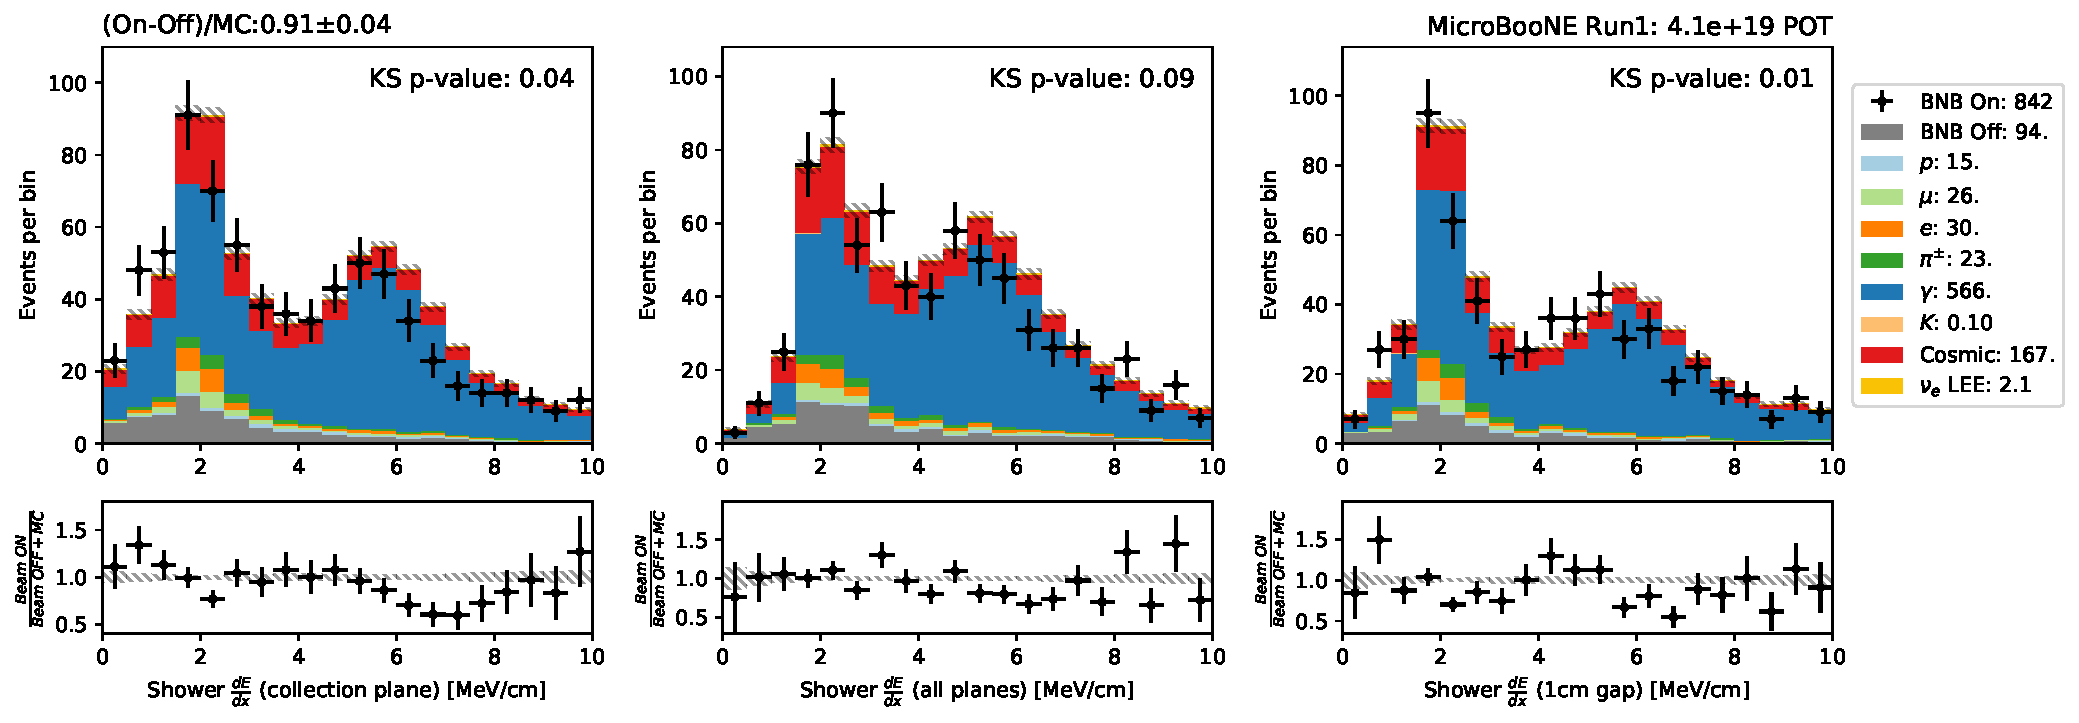
\includegraphics[width=\textwidth]{NueCCsel/Images/run1/e_cand_dedx.pdf}
    \caption{d$E$/d$x$ of the electron candidate shower after the pre-selection. The collection plane shows the cleanest e/$\gamma$ separation. The middle panel combines all three planes, leading to a smaller peak at 0 in cases where there are few hits on the collection plane. The plane on the right uses the collection plane but leaves a \SI{1}{\cm} gap, which is beneficial when vertex activity is merged into the electron shower.}
    \label{fig:e_cand_dedx}
\end{figure}

\begin{figure}
    \centering
    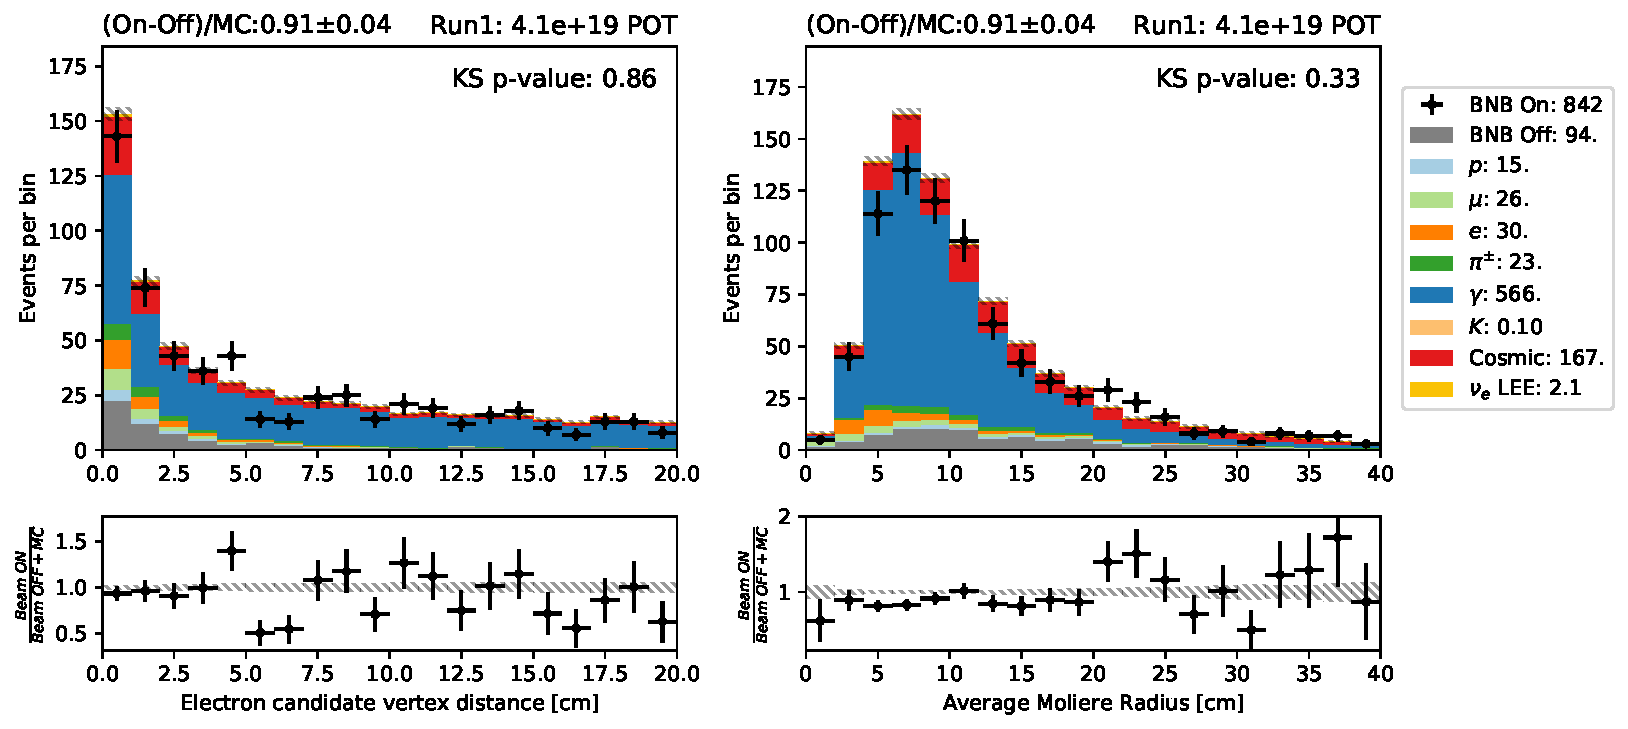
\includegraphics[height=5cm]{NueCCsel/Images/run1/e_cand_dist.pdf}
    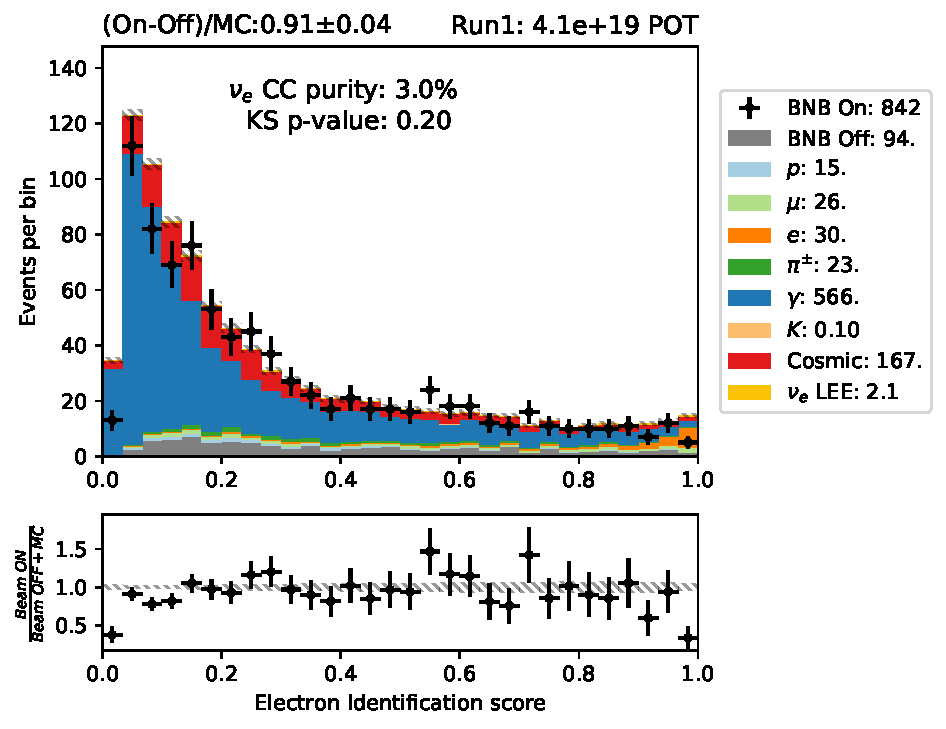
\includegraphics[height=5cm]{NueCCsel/Images/run1/pre_e_score.pdf}
    \caption{The left two panels show important variables to identify electrons after the pre-selection. The right panel shows the BDT elctron identification response, demonstrating a good e/$\gamma$ separation.}
    \label{fig:e_cand_dist}
\end{figure}

%\begin{figure}
%    \centering
%    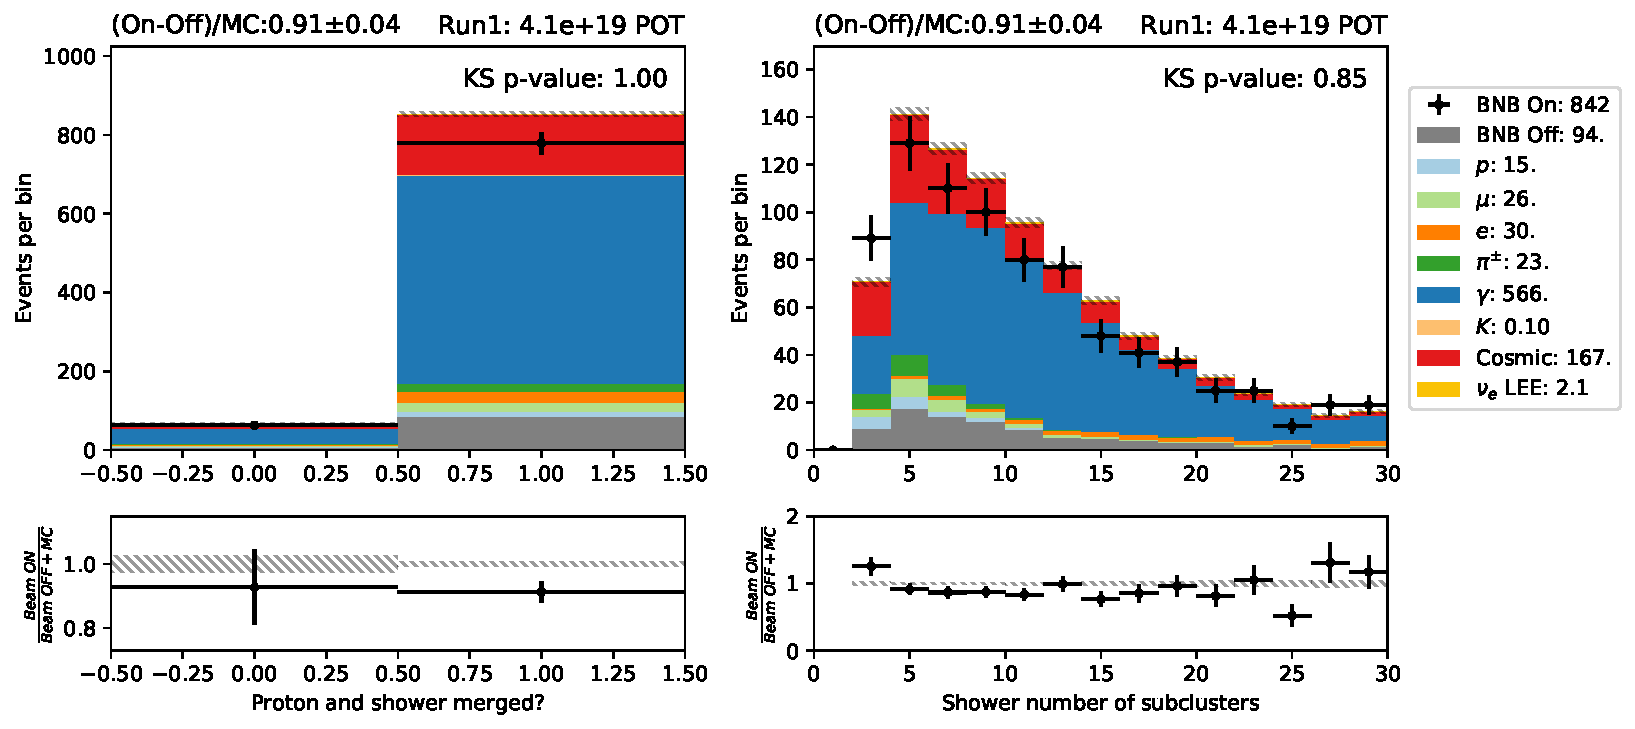
\includegraphics[width=\textwidth]{NueCCsel/Images/run1/e_cand_subclusters.pdf}
%    \caption{Caption}
%    \label{fig:e_cand_subclusters}
%\end{figure}

%\begin{figure}
%    \centering
%   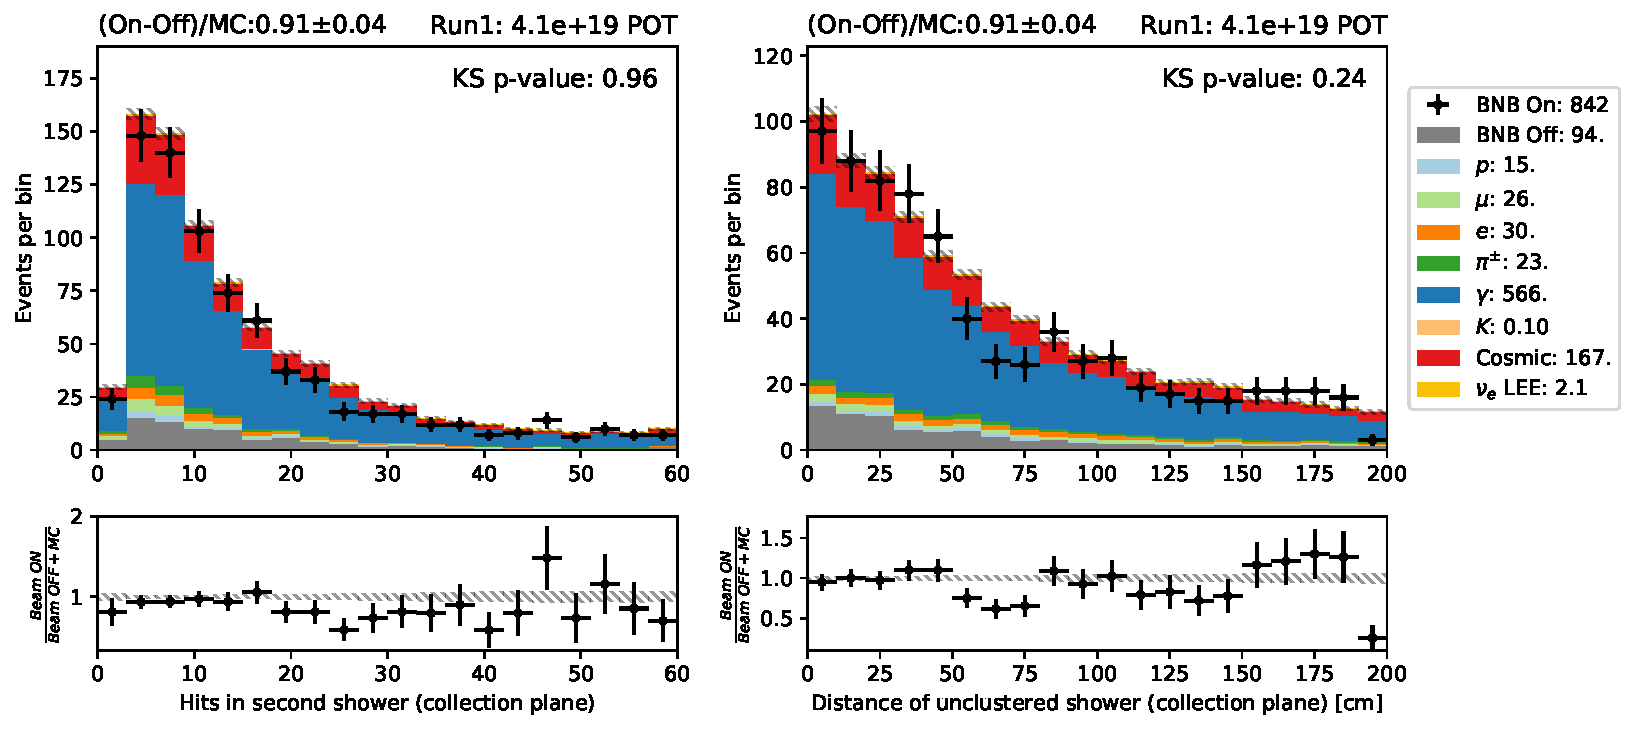
\includegraphics[width=\textwidth]{NueCCsel/Images/run1/e_cand_secondshower.pdf}
%    \caption{Caption}
%    \label{fig:e_cand_secondshower}
%\end{figure}

\subsubsection{Other Daughters Identification}

Apart of the electron candidate particle, there are other particles in the slice. These tracks and showers can be part of the $\nu_e$ CC event, but they can also help us to identify the event as background. The event should not contain a particle backtracked to cosmic overlay activity or simulated muons. On the other hand, particles that correspond to protons or split off parts of the electron shower should not lead to the rejection of the event. The more complicated situation arises when pions are present. Charged pions should be allowed in a $\nu_e$ CC search, but the mis-identification rate between charged pions and muons is large in this detector type. Photons coming from neutral pions, appart of the electron shower candidate, can be part of the $\nu_e$ CC event, but can also help to reduce the NC $\pi^0$ backgrounds. It was chosen therefore to not use pions in the BDT training and give them a neutral label. The input variables of the BDT are:
\begin{enumerate}
    \item trk\_llr\_pid\_score
    \item trk\_distance
    \item trk\_score
    \item The generation of the particle: primary daughter of the neutrino or secondary.
    \item Has the particle a shower or a track as daughter?
\end{enumerate}
The three most important distributions of the variables used are given in \cref{fig:pre_daughter_1}. The response of the BDT is shown in \cref{fig:pre_daughter_score}.


\begin{figure}
    \centering
    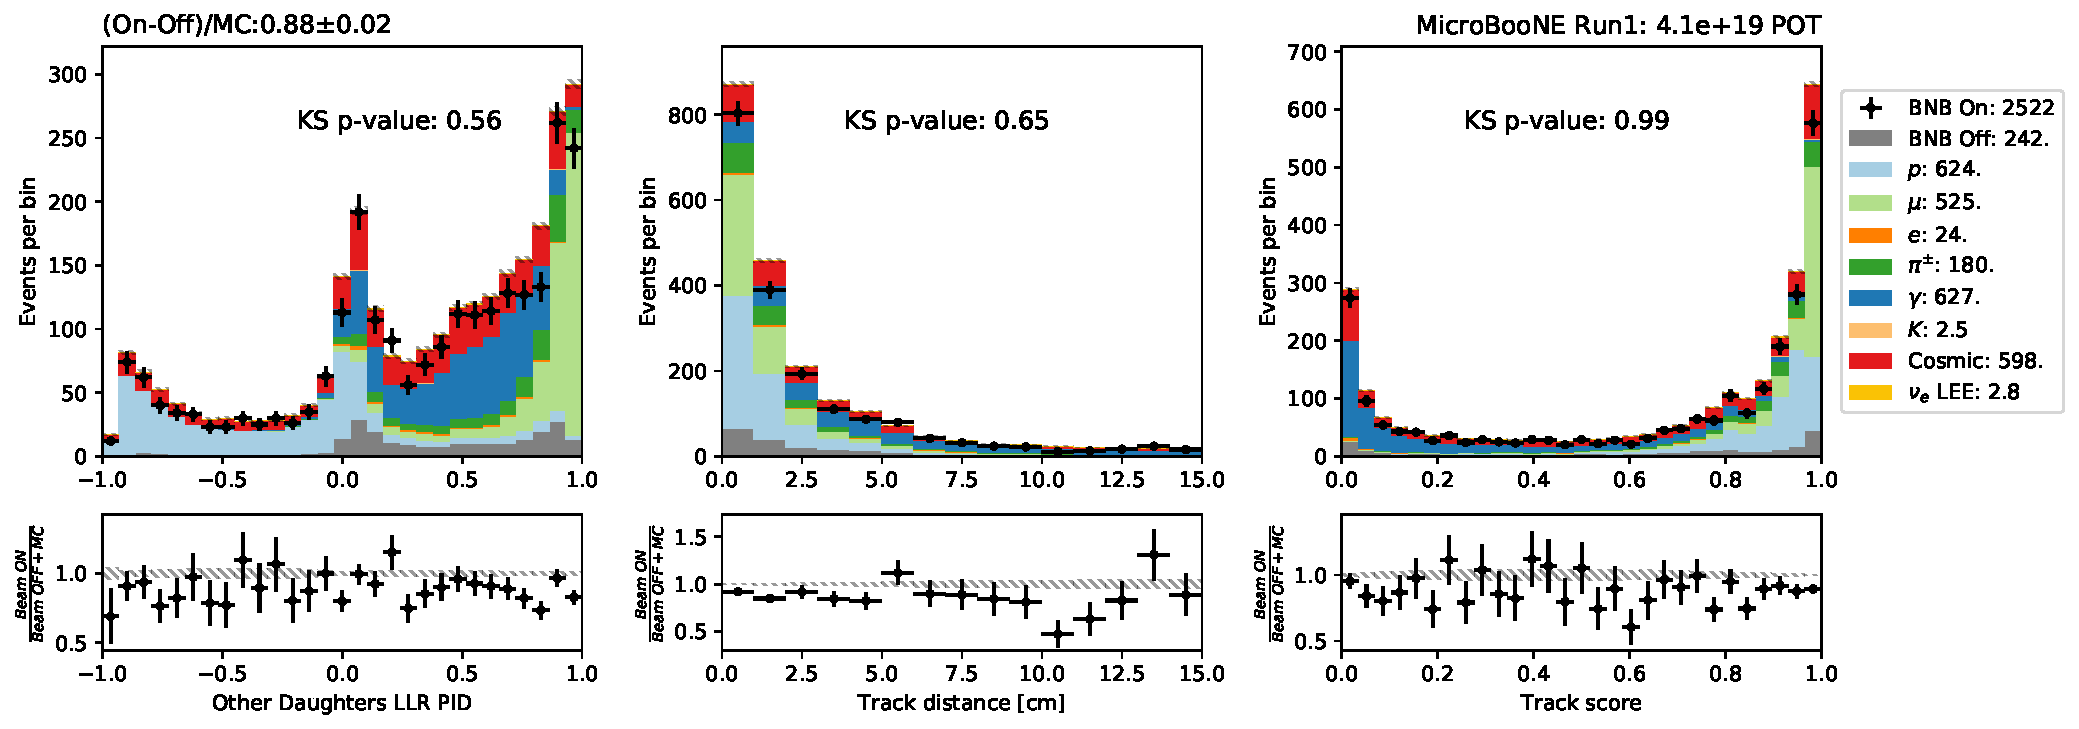
\includegraphics[width=\textwidth]{NueCCsel/Images/run1/pre_daughter_1.pdf}
    \caption{Variables used to identify the other daughters of the neutrino besides the electron candidate shower. The distributions include all non-electron tagged daughters after the pre-selection.}
    \label{fig:pre_daughter_1}
\end{figure}

%\begin{figure}
%    \centering
%    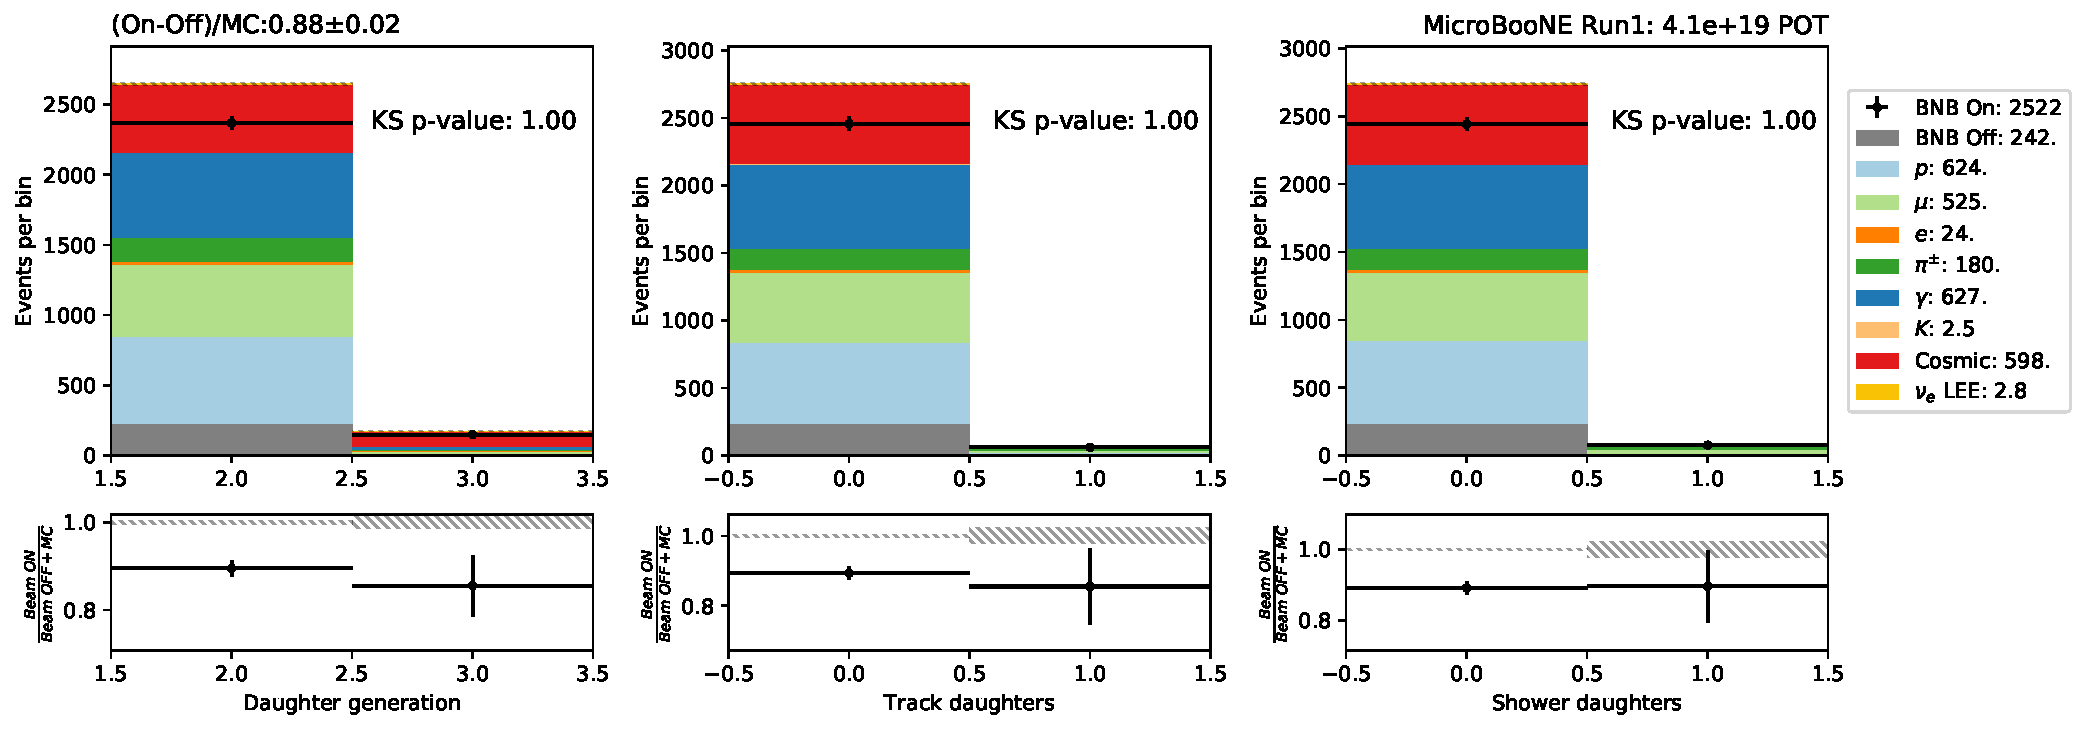
\includegraphics[width=\textwidth]{NueCCsel/Images/run1/pre_daughter_2.pdf}
%    \caption{Caption}
%    \label{fig:pre_daughter_2}
%\end{figure}

\begin{figure}
    \centering
    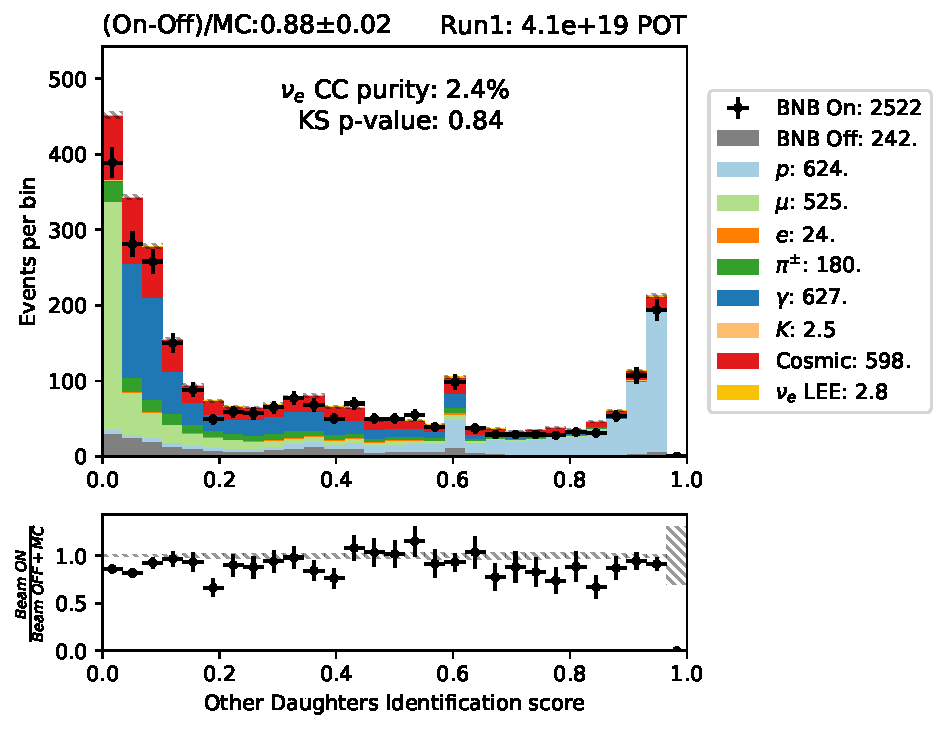
\includegraphics[width=0.5\textwidth]{NueCCsel/Images/run1/pre_daughter_score.pdf}
    \caption{BDT response to classify the non-electron candidate daughters in the event. The cosmogenic particles, together with the muons and photons have a low response, indicating higher likeliness to be background. The protons have a high response on the right.}
    \label{fig:pre_daughter_score}
\end{figure}

\subsubsection{Event Selection}
The final event classification build on top of the particle identification performed in the two previous sections. THe dominating variable is the electron identification response but the full list of variables is, in sequence of importance:

\begin{enumerate}
    \item Electron BDT response
    \item Lowest BDT response of the other daughter BDT
    \item contained\_fraction
    \item Number of showers
    \item hits\_ratio
    \item Mean BDT response of the other daughter BDT
    \item Number of particles away from the vertex.
\end{enumerate}
The response of the event classification is given in the left panel \cref{fig:pre_event_score}. After the selection, the efficiency is 21\%, corresponding to 280 electron neutrino's in the Run 1-4 data-set. The distribution of the reconstructed electron energy is given in the right panel of \cref{fig:pre_event_score}. \cref{fig:nueccinc_eff} documents the efficiency of the SliceID, pre-selection and final inclusive selection for the three final state categories.

%\begin{figure}
%    \centering
%    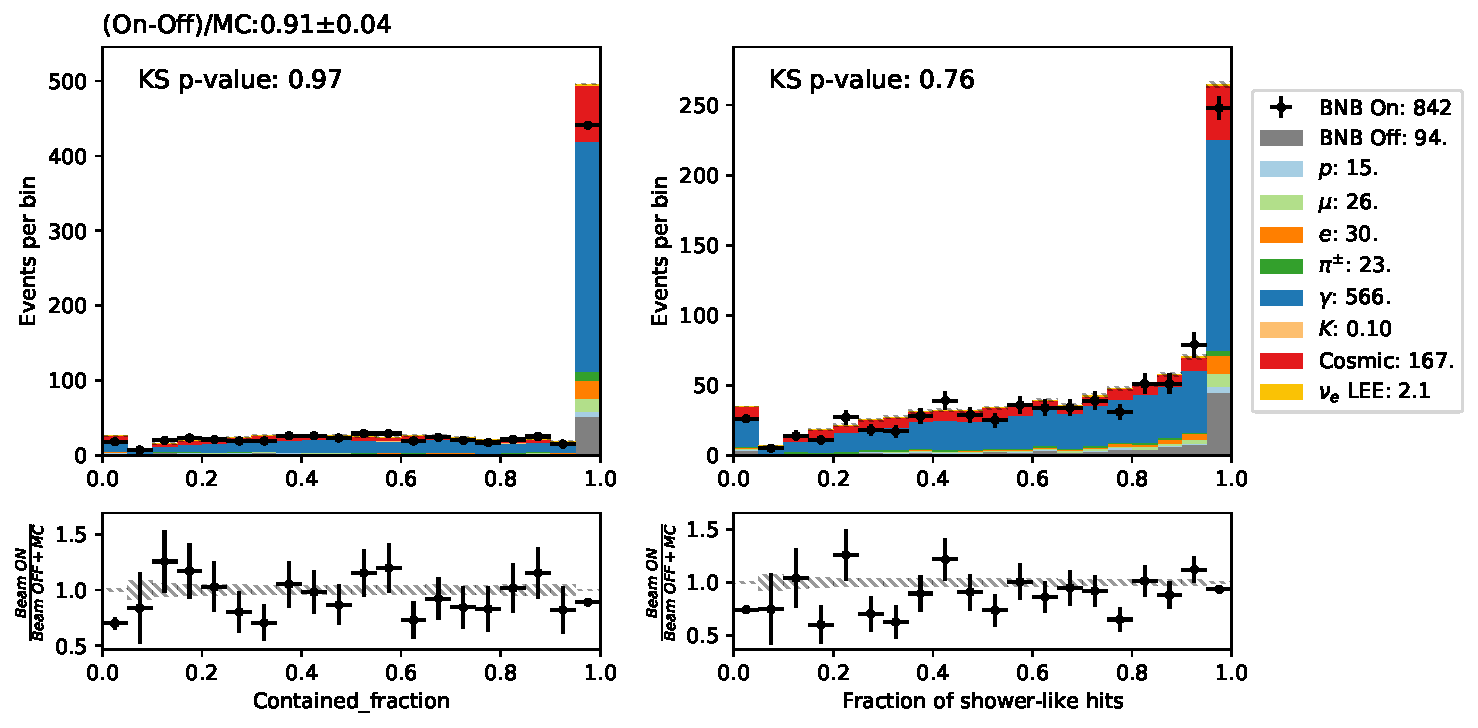
\includegraphics[width=\textwidth]{NueCCsel/Images/run1/bdt_1.pdf}
%    \caption{Caption}
%    \label{fig:bdt_1}
%\end{figure}

%\begin{figure}
%    \centering
%    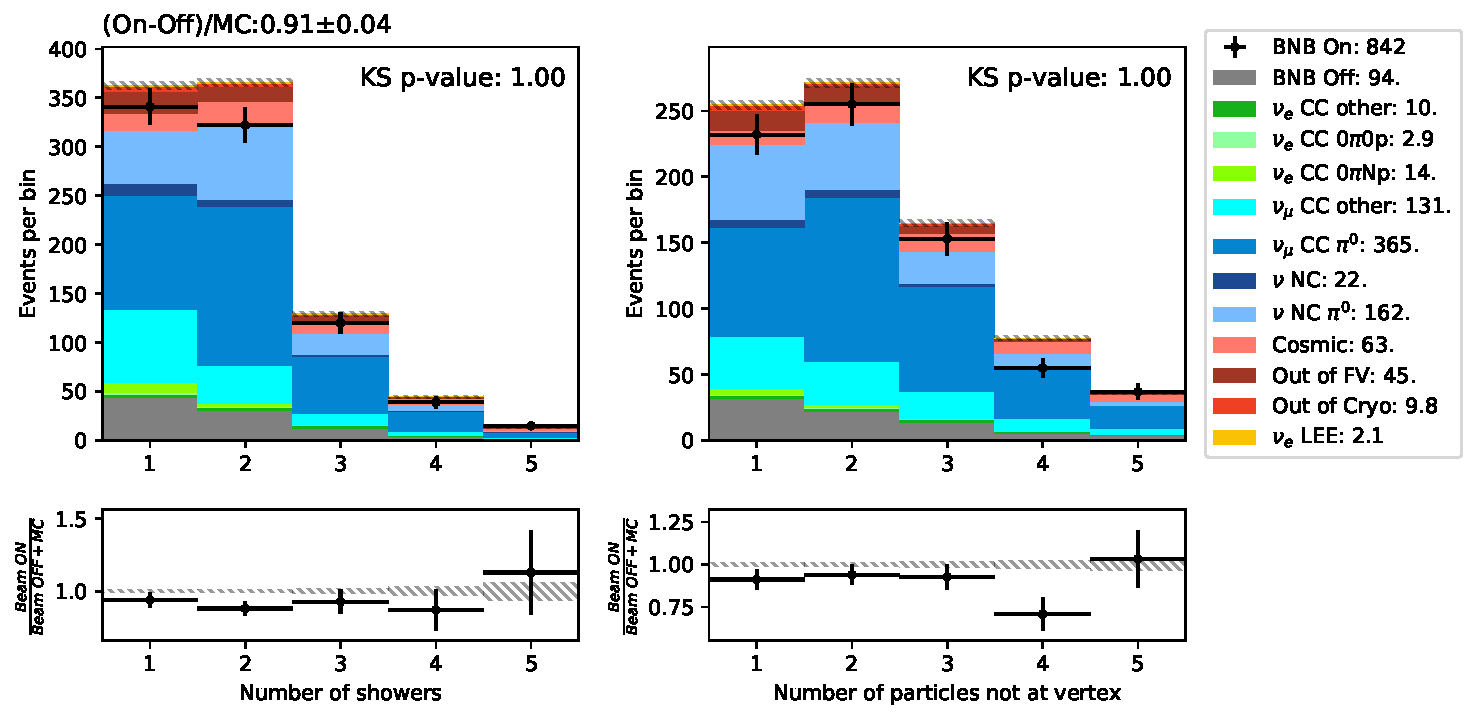
\includegraphics[width=\textwidth]{NueCCsel/Images/run1/bdt_2.pdf}
%    \caption{Caption}
%    \label{fig:bdt_2}
%\end{figure}

\begin{figure}
    \centering
    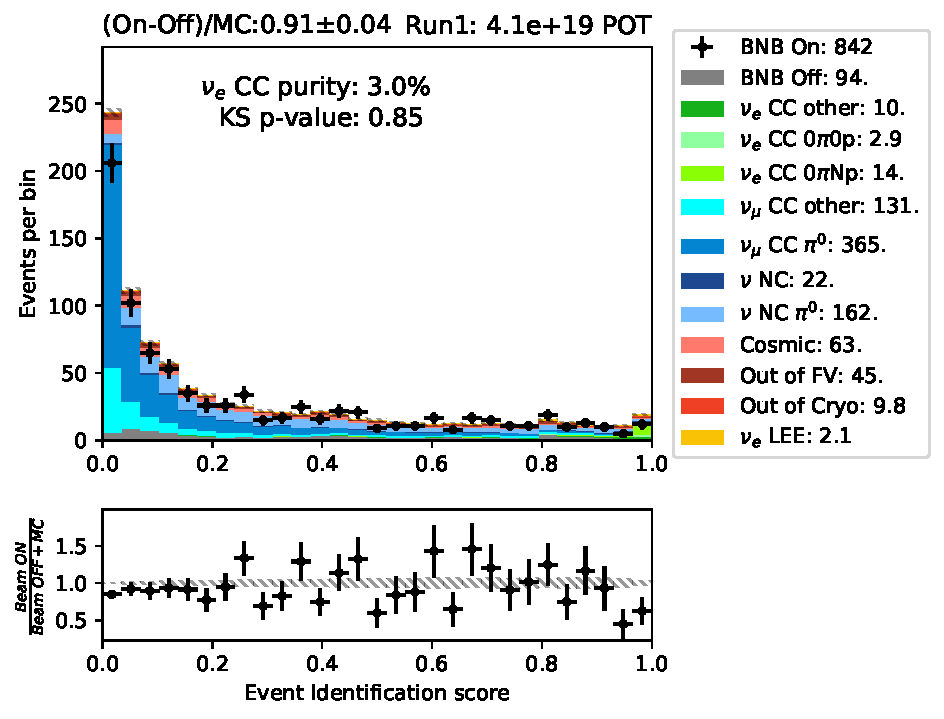
\includegraphics[width=0.445\textwidth]{NueCCsel/Images/run1/pre_event_score.pdf}
    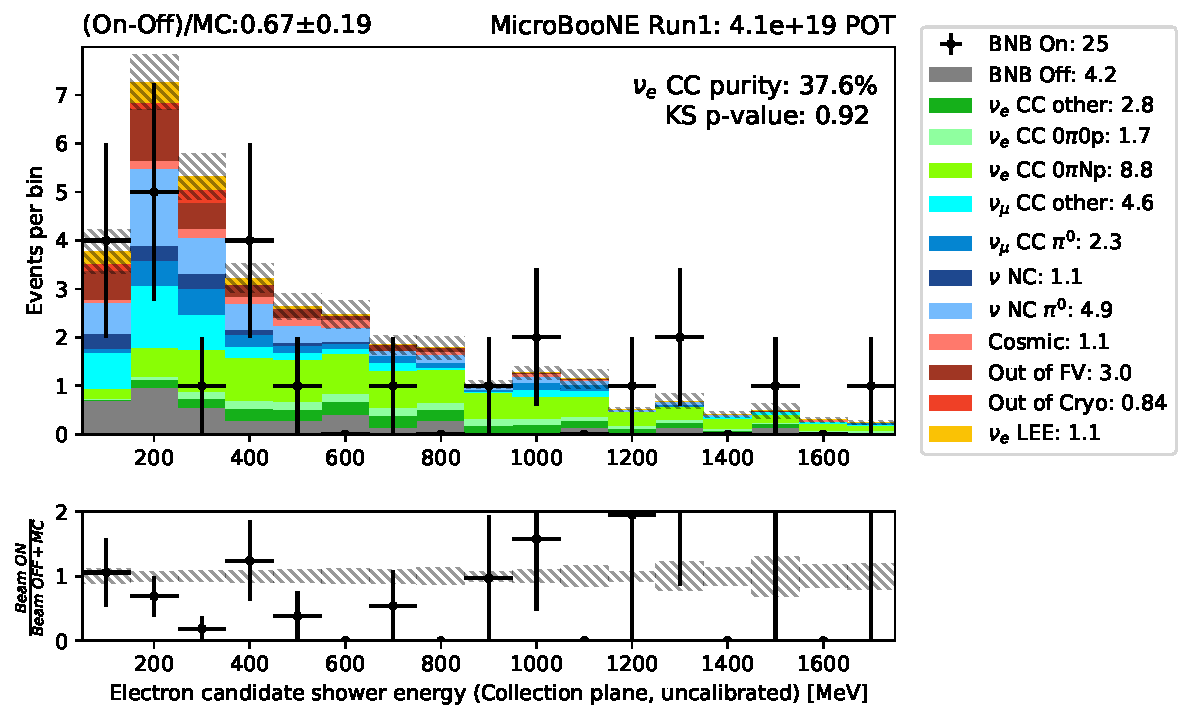
\includegraphics[width=0.545\textwidth]{NueCCsel/Images/run1/nue_shower_energy_y.pdf}
    \caption{(left) BDT response of the $\nu_e$ CC inclusive event classifier. (right) Electron shower energy distribution after the selection.}
    \label{fig:pre_event_score}
\end{figure}

\begin{figure}
    \centering
    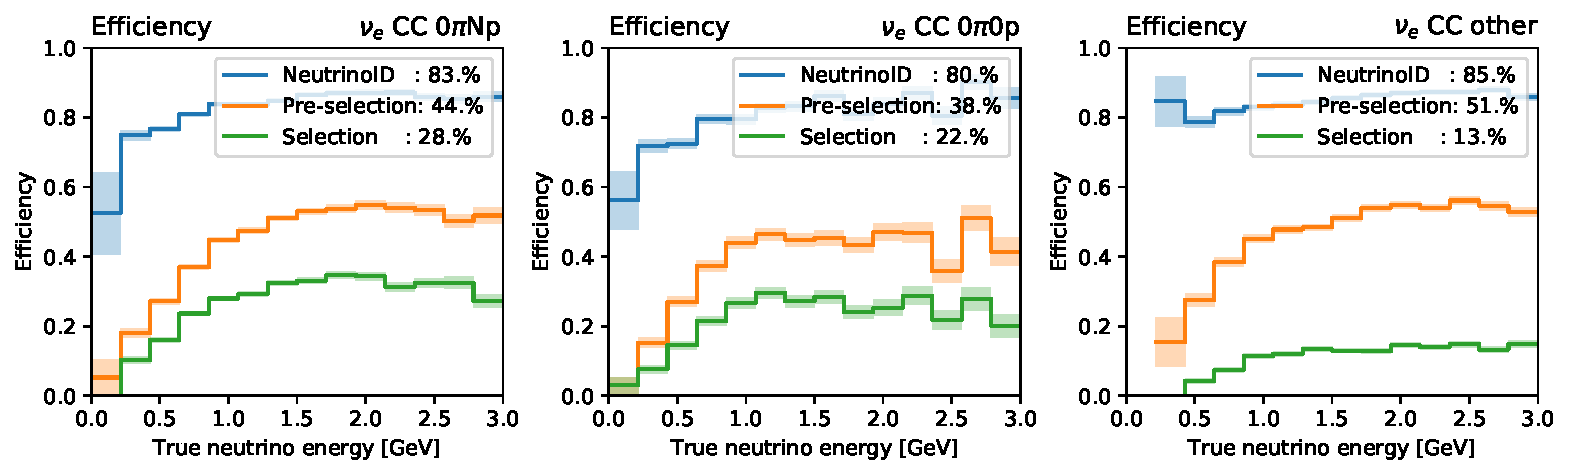
\includegraphics[width=\textwidth]{NueCCsel/Images/run1/efficiency_cat_2.pdf}
    \caption{Efficiency of the different stages in the selection in function of the true neutrino energy. The different panels correspond to different final states of interest.}
    \label{fig:nueccinc_eff}
\end{figure}

